\documentclass[modern]{aastex62}

% Load the corTeX style definitions
% All the packages
\usepackage{url}
\usepackage{amsmath}
\usepackage{mathtools}
\usepackage{amssymb}
\usepackage{natbib}
\usepackage{graphicx}
\usepackage{calc}
\usepackage{etoolbox}
\usepackage{xspace}
\usepackage[T1]{fontenc} % https://tex.stackexchange.com/a/166791
\usepackage{textcomp}
\usepackage{ifxetex}
\ifxetex
\usepackage{fontspec}
\defaultfontfeatures{Extension = .otf}
\fi
\usepackage{fontawesome}
\usepackage{listings}

% Shorthand for this paper
\newcommand{\Python}{\textsf{Python}\xspace}
\newcommand{\cpp}{\textsf{C}++\xspace}
\newcommand{\starry}{\textsf{starry}\xspace}
\newcommand{\spiceypy}{\textsf{spiceypy}\xspace}
\newcommand{\tf}{\textsf{TensorFlow}\xspace}
\newcommand{\tess}{\emph{TESS}\xspace}

% References to text content
\newcommand{\documentname}{\textsl{article}}
\newcommand{\figureref}[1]{\ref{fig:#1}}
\newcommand{\Figure}[1]{Figure~\figureref{#1}}
\newcommand{\figurelabel}[1]{\label{fig:#1}}
\renewcommand{\eqref}[1]{\ref{eq:#1}}
\newcommand{\Eq}[1]{Equation~(\eqref{#1})}
\newcommand{\eq}[1]{\Eq{#1}}
\newcommand{\eqalt}[1]{Equation~\eqref{#1}}

% Add code, proof, and animation hyperlinks
\definecolor{linkcolor}{rgb}{0.1216,0.4667,0.7059}
\newcommand{\codeicon}{{\color{linkcolor}\faFileCodeO}}
\newcommand{\prooficon}{{\color{linkcolor}\faPencilSquareO}}
\newcommand{\codelink}[1]{\href{https://github.com/rodluger/earthshine/blob/3b1b4e288b46cb8823ff70e269c2acbf3303b236/notebooks/#1.ipynb}{\codeicon}\,\,}


% Define a proof environment for open source equation proofs
\newtagform{eqtag}[]{(}{)}
\newcommand{\currentlabel}{None}
\newenvironment{proof}[1]{%
\ifstrempty{#1}{%
\renewtagform{eqtag}[]{\raisebox{-0.1em}{{\color{red}\faPencilSquareO}}\,(}{)}%
}{%
\renewtagform{eqtag}[]{\prooflink{#1}\,(}{)}%
}%
\usetagform{eqtag}%
\renewcommand{\currentlabel}{#1}
\align%
}{%
\endalign%
\renewtagform{eqtag}[]{(}{)}%
\usetagform{eqtag}%
\message{<<<\currentlabel: \theequation>>>}%
}

% Define the `oscaption` command for open source figure captions
\newcommand{\oscaption}[2]{\caption{#2 \codelink{#1}}}

% Code examples
\definecolor{codegreen}{rgb}{0,0.6,0}
\definecolor{codegray}{rgb}{0.5,0.5,0.5}
\definecolor{codepurple}{rgb}{0.58,0,0.82}
\definecolor{backcolour}{rgb}{0.95,0.95,0.95}
\lstdefinestyle{mystyle}{
    backgroundcolor=\color{backcolour},
    commentstyle=\color{codegreen},
    keywordstyle=\color{magenta},
    numberstyle=\tiny\color{codegray},
    stringstyle=\color{codepurple},
    basicstyle=\small\ttfamily,
    breakatwhitespace=false,
    breaklines=true,
    captionpos=b,
    keepspaces=true,
    numbers=left,
    numbersep=5pt,
    showspaces=false,
    showstringspaces=false,
    showtabs=false,
    tabsize=2,
    aboveskip=1em,
    belowskip=1em,
    keywords=[2]{map},
    keywordstyle=[2]{\color{black!80!black}},
    upquote=true
}
\lstset{style=mystyle}

% Typography obsessions
\setlength{\parindent}{3.0ex}
\renewcommand\quad{\hskip\fontdimen3\font}


\usepackage{xcolor}
\usepackage{xspace}
\newcommand{\TESS}{\emph{TESS}\xspace}
\newcommand{\todo}[1]{\textcolor{red}{#1}}

% Bibliography stuff
\bibliographystyle{aasjournal}

% Begin!
\begin{document}

% Title
\title{\TESS Photometric Mapping of a Terrestrial Planet in the Habitable Zone: 
       Detection of Clouds, Oceans, and Continents}
%\title{Detection of Continents on a Habitable-Zone Terrestrial Planet with \TESS}

% Author list
\author[0000-0002-0296-3826]{Rodrigo Luger}
\email{rluger@flatironinstitute.org}
\affil{Center~for~Computational~Astrophysics, Flatiron~Institute, New~York, NY}
%
\author[0000-0002-9328-5652]{Megan Bedell}
\affil{Center~for~Computational~Astrophysics, Flatiron~Institute, New~York, NY}
%
\author{Roland K. Vanderspek}
\affil{Kavli Institute for Astrophysics and Space Research, Massachusetts 
       Institute of Technology, Cambridge, MA}
%
\author{Christopher J. Burke}
\affil{Kavli Institute for Astrophysics and Space Research, Massachusetts 
       Institute of Technology, Cambridge, MA}

\begin{abstract}
\todo{[maybe change first sentences to focus on planet mapping \& give the game 
away less?]} The Transiting Exoplanet Survey Satellite (\TESS) mission is a 
targeted effort to detect planets smaller than Neptune around bright, nearby stars. 
While \TESS is already enjoying great success with the discovery of many new worlds, 
the strongest signal in its data is typically ignored, as it lurks in the background 
of every camera pixel. In this work, we extract this signal and demonstrate that 
it is consistent with a terrestrial planet with a rotation period of 1 day. 
Using a spherical harmonic-based reflection model developed as an extension of 
the \starry package, we are able to reconstruct the surface features of this rocky 
world. We recover a time-variable albedo map of the planet including persistent 
regions which we interpret as continental features and cloud banks. 
We argue that this planet represents the most promising detection of a habitable 
world to date, although the potential intelligence of any life on it is yet to 
be determined.
\end{abstract}

\keywords{methods: data analysis, techniques: photometric, planets and satellites: 
          oceans, planets and satellites: surfaces, planets and satellites: 
          terrestrial planets}

% Introduction
\section{Introduction}
\label{sec:intro}

%Resolving the features of planetary atmospheres and surfaces with precise 
%photometry is a crucial 
Precise photometry obtained over long periods of time can reveal the atmospheric 
and surface features of an exoplanet through the method known as phase mapping. 
\todo{(literature background \& citations)}

A new source of precise photometry is the Transiting Exoplanet Survey Satellite 
\citep[\TESS; ][]{Ricker2015}. 
Launched in April 2018, \TESS has... \todo{(summary of \TESS's capabilities, 
citations to planet discoveries etc)}

One intriguing feature of the \TESS photometric data products is a highly 
time-variable signal represented in the diffuse background across virtually 
all camera pixels. 
\todo{(talk abt Earthshine without naming it)} 
The signal has been widely attributed to a planet which we will call Sol d.

Previous attempts to map this planet from the exoplanet community have suggested 
the presence of localized surface features, but their resolving power has been 
severely limited by the duration of observations \citep{Cowan2009}. 
\TESS offers precise 2-minute cadence data spanning a wide range of illumination 
phases, enabling a level of spatial and temporal resolving power that is 
unprecedented in the exoplanetary phase mapping literature. 

Moreover, recent advances in fast analytic computation of spherical harmonics 
have made the reconstruction of such detailed maps more feasible than ever. 
\todo{(STARRY)}

In this work, we build on this methodological foundation to perform 
reflected-light mapping of planetary surface features on Sol d. 
We give an overview of the \TESS data used in Section \ref{sec:data}. 
In Section \ref{sec:methods}, we describe the methods employed to infer a map 
from these data, including the adaptation of the \starry algorithm to reflection 
mapping, the modeling of spacecraft-related systematics, and the likelihood and 
priors used. 
We present results in Section \ref{sec:results} and make comparison of these 
findings to state-of-the-art terrestrial planet maps from the literature in 
Section \ref{sec:discussion}. 
Finally, we conclude in Section \ref{sec:conclusion} with a look at future 
prospects for phase-curve mapping of terrestrial exoplanets.

\section{Data}
\label{sec:data}

The \TESS pipeline produces processed lightcurves for all short-cadence targets. 
Part of this processing is the determination of the localized background flux within each postage stamp, which is provided as an ancillary time series. 
As with all \TESS time series data products, the time is given in \TESS Julian Days (TJD), defined as BJD - 2457000, and the data are delivered in 27-day parcels corresponding to the varying pointing sectors of \TESS. 
We use these background flux measurements from Sectors 1 and 2 as our primary data source in this work. 

For each of the two sectors considered, we downloaded a randomized subsample of 1000 short-cadence lightcurve files corresponding to postage stamps located across the full \TESS field of view and extracted the background flux time series from each. 
Not all postage stamps are equally informative, since the desired signal from Sol d is inhomogenously spread across the \TESS detectors and manifests differently in different regions (see Section \ref{sec:systematics}). 
We down-selected our pool of 1000 targets to 75 maximally useful background lightcurves from Sector 1 and 20 from Sector 2. 
This down-selection was done with several criteria in mind: each lightcurve should contain a significant signal from Sol d; they should be representative of the general background flux modulation seen across the \TESS cameras, rather than containing any truly localized signals from astrophysical background sources; and the sample as a whole should contain the full range of typical behaviors of background across the entire \TESS field of view. 
To accomplish this, we... \todo{(decide whether it's outlier rejection only or full-on categorization)}

\todo{(masking out epochs without Sol d shine, subtraction of baseline background flux)}

The final data set to be used consists of 75 Sector 1 background lightcurves and 20 Sector 2 background lightcurves corresponding to the epochs at which Sol d signal was clearly registered by \TESS. 
This is 912,605 data points in total. 
A representative sample of these signals is shown in Figure~\ref{fig:data}.

\begin{figure}[t!]
    \begin{centering}
    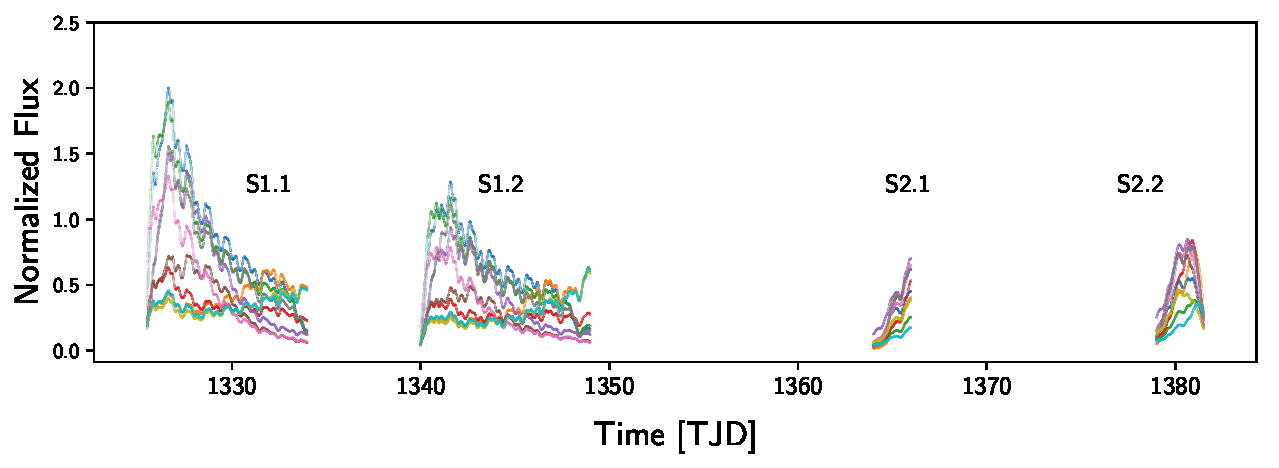
\includegraphics[width=\linewidth]{figures/data.pdf}
    \caption{\label{fig:data}
             Normalized background flux in each of ten postage stamps
             for each of Sectors 1 and 2. Cadences where Sol d was
             below or very close to the edge of the sunshade were masked.
             While the planet is in view for the majority of both orbits
             in Sector 1, it is only visible in the data at the very end
             of each orbit in Sector 2.
             \codelink{earthshine_S1_S2}
             }
    \end{centering}
\end{figure}

\section{Methods}
\label{sec:methods}

\subsection{Orbital Modeling}
\label{sec:orbit}

We downloaded 
\footnote{\url{https://archive.stsci.edu/missions/tess/models/}}
the Solar System and \tess ephemeris data for
Sectors 1 and 2 and used \spiceypy \citep{Acton1996, Acton2017, Annex2017}
to convert the TJD timestamps to 
ephemeris time (ET). We then used the \textsf{spkezr} utility of \spiceypy to compute
the relative positions of Sol, Sol d, and \tess for every cadence
in our dataset in the J2000 equatorial reference frame. In this right-handed
coordinate frame, Sol d is centered at the origin, the $y$ axis points along the 
planet's spin axis, and the $x$ axis points toward the vernal equinox. We
do not apply any light travel correction, as the expected delay is on the order
of a few seconds.

At any given cadence, we rotate Sol d about its spin axis to the correct phase,
assuming a rotation period of $0.9972696$ day, the sidereal rotation period
of the planet. We determine the initial rotation
phase of Sol d by computing the Sol d Rotation Angle (ERA), given by \citep{Urban2013}
%
\begin{align}
\mathrm{ERA} = 360^\circ(0.7790572732640 + 1.00273781191135448 \, t_U) \, \mathrm{mod} \, 360^\circ
\end{align}
%
where $t_U = t - 2451545.0$. At $t = t_0 = 2458325.5$, the first timestamp in our dataset,
we find $\mathrm{ERA} = 303.4^\circ$, meaning the vernal equinox will be aligned with
the prime meridian $360^\circ - 303.4^\circ = 56.6^\circ = 3.77$ hours past $t_0$.
%
Finally, we rotate the frame to align
\tess with the $+z$ axis, with the spin vector of Sol d along the $y-z$ plane.
We verified our rotations by comparing our results on several days to the
ephemerides provided by the JPL HORIZONS Web interface%
\footnote{See \url{https://ssd.jpl.nasa.gov/horizons.cgi} and 
\href{https://github.com/rodluger/earthshine/blob/master/notebooks/SanitCheck.ipynb}{this
Jupyter notebook.}}.

\begin{figure}[t!]
    \begin{centering}
    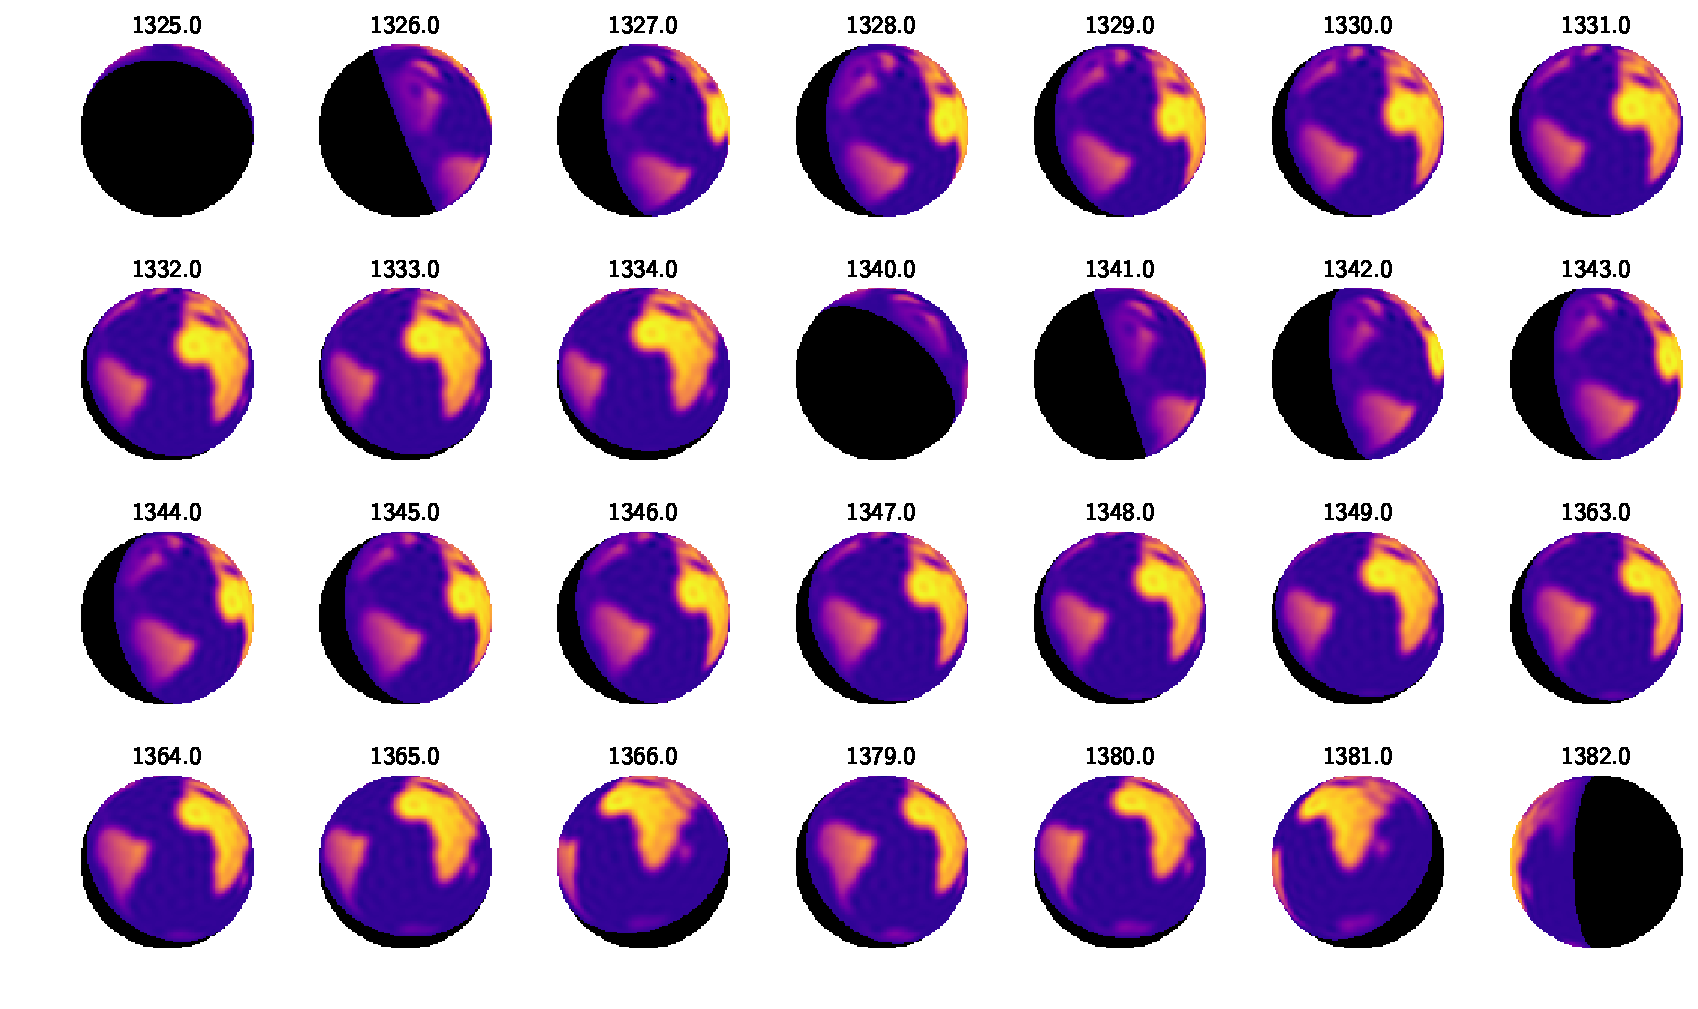
\includegraphics[width=\linewidth]{figures/phases.pdf}
    \caption{\label{fig:phases}
             \tess view of Sol d on every date in Sectors 1
             and 2 that was included in the regression. Each image is
             labeled with the corresponding timestamp in TJD. The images
             shown here correspond to current models of the continental coverage
             of Sol d, not to the map inferred in this study.
             \codelink{EarthView}
             }
    \end{centering}
\end{figure}

Figure~\ref{fig:phases} shows the view \tess has of Sol d on each of the dates
in our dataset; these images were produced by applying the sequences of rotations
described above. The planet is illuminated by Sol assuming it is a point source,
and the night side is shaded black. The map of Sol d shown in this figure is 
based on current models of the actual distribution of continents on the planet.
Note that although the images are computed an integer number of rotation periods
apart, the planet appears to slowly rotate over the course of the observation.
This is because of the orbit of \tess, which changes its vantage point relative
to Sol d over the course of its 13 day orbit.

\subsection{Systematics Modeling}
\label{sec:systematics}

While the astrophysical signal that we wish to analyze is present in all 
extracted lightcurves, its strength is modulated by time-variable systematics 
that are correlated but not identical across all postage stamps, since the
illumination of the CCD by Sol d is strongly inhomogeneous. A physical
model of the reflections and scattering that gives rise to the
signal of Sol d on the \tess detector is beyond the scope of this work. Instead,
we treat this as a de-trending problem, where the signal we wish to fit is
shared by all postage stamps, but multiplied by a systematic signal that is
different for each target. This problem is precisely what the technique of
pixel-level decorrelation \citep[PLD;][]{Deming2015, Luger2016, Luger2018a}
seeks to address. In PLD, one computes the sum over all light curves at each
point in time, and uses this quantity to normalize each of the individual
light curves. Since (by assumption) each light curve is the product of the astrophysical
signal and the systematics signal, this procedure divides out the astrophysical
signal, producing a basis of vectors that contain \emph{only} functions of the
systematics. This now serves as a ``clean'' basis one can then use to fit the
data, with minimal risk of fitting out astrophysical signals.

We therefore construct a design matrix $\mathbf{B}$ out of the PLD basis. To
increase the flexibility of the systematics model, we append to $\mathbf{B}$ 5 orthogonal
polynomials in time for each of the two orbits of \tess in each sector.
The systematics model $\mathbf{p}$ for the $n^\mathrm{th}$ signal is thus
%
\begin{align}
\mathbf{p}_n = \mathbf{B} \mathbf{w}_n
\end{align}
%
where $\mathbf{w}_n$ are the weights of each regressor.
Since we solve for different weights for each of the 75 light curves in Sector 1
and 20 light curves in Sector 2, our systematics model has
$75 \times (75 + 2 \times 5) + 20 \times (20 + 2 \times 5) = 6,975$ free parameters.
The total number of data points is $912,605$, so overfitting is not particularly
concerning; nevertheless, we impose an L2 prior on the weights with
standard deviation $\sigma_B = 0.1$ (see \S\ref{sec:model}).

\subsection{Reflected Light Mapping with \starry}
\label{sec:starry}

We model the astrophysical component of the signal---the rotational modulation
of Sol d in reflected light---using the \starry code package \citep{Luger2019}.
\starry computes phase curves and occultation light curves for bodies whose
surfaces are expressed as a sum of spherical harmonics. 
The algorithm works by first transforming
from spherical harmonic coefficients to coefficients in the polynomial basis $\tilde{p}$, whose
terms are of the form $x^i y^j z^k$ for (non-negative) integer $i$ and $j$ 
and $k = 0$ or $1$. \citet{Luger2019} showed how to compute the visible
flux by integrating each of the terms in $\tilde{p}$ across the visible
surface of the projected disk. For unocculted spheres observed in emitted
light, the area of integration is the full disk, which makes the integration
trivial: the flux contribution from each term in $\tilde{p}$ is a constant
easily computed via recursion relations involving factorials. The algorithm is
thus extremely fast and very precise.

However, in the present work, we are interested in \emph{reflected} light, so we must
account for the illumination by the star, which varies smoothly
across the dayside of the planet but whose derivative discontinuously changes at the 
terminator, beyond which the illumination is zero everywhere. This requires
two modifications to the \starry algorithm: we must (1) weight all integrands
by the illumination function on the dayside, and (2) modify the integration
limits to truncate the integrals at the day/night terminator.

\begin{figure}[t!]
    \begin{centering}
    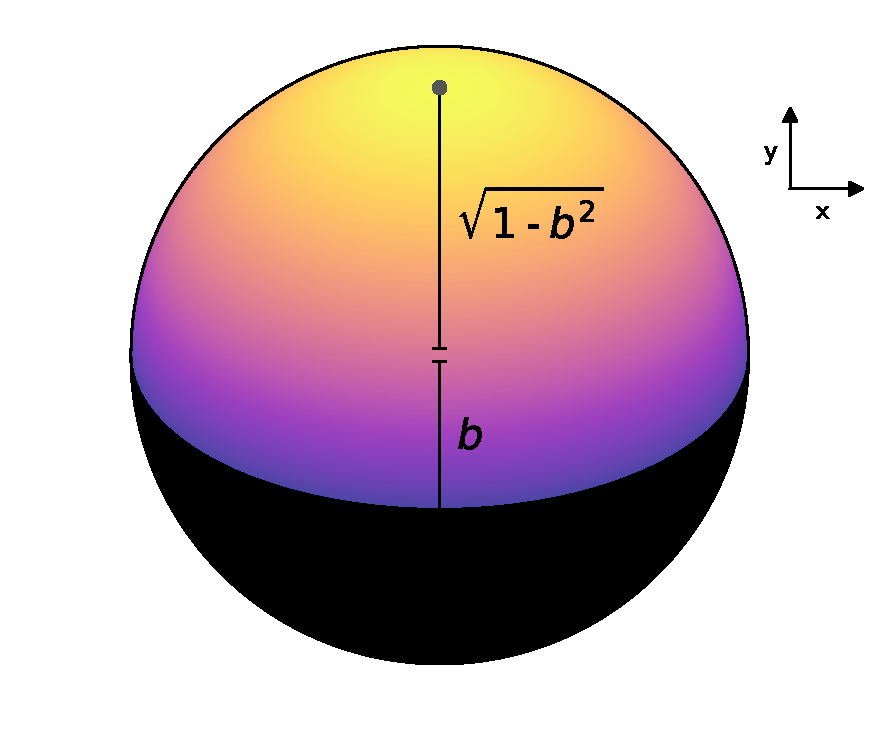
\includegraphics[width=0.4\linewidth]{figures/geometry.pdf}
    \caption{\label{fig:geometry}
             Geometry of the \starry model in reflected light. In this frame, 
             the $y$ axis points up, 
             the $x$ axis points to the right, and the $z$ axis points out of the page.
             The planet has unit radius and sits at the origin, while
             the illumination source is along the $y-z$ plane, with the sub-stellar point is
             marked by a dot. The semi-major axis of the terminator is unity, and
             the semi-minor axis of the terminator is denoted $b$. The night side
             is colored black.
             \codelink{Geometry}
             }
    \end{centering}
\end{figure}

Let us consider a right-handed coordinate frame in which the planet has unit 
radius and is located at the origin, the illumination source is along the $y-z$
plane, and the sub-stellar point is on the $+y$ axis at $x = 0$
(see Figure~\ref{fig:geometry}). In this frame, the terminator is a segment of
an ellipse, with semi-major axis $a=1$ aligned with the $x$ axis and
semi-minor axis $b$. It is straightforward to show that the sub-stellar point
is located at $y=\sqrt{1 - b^2}$ and the illumination is given by
%
\begin{align}
    I(b; x, y) &= 
    \begin{dcases}
        \sqrt{1 - b^2}y - bz & 
            \quad\quad\quad\quad\quad\quad\quad\quad\quad\quad 
            y \geq -b \sqrt{1 - x^2}
        \\
        0 & 
            \quad\quad\quad\quad\quad\quad\quad\quad\quad\quad 
            \mathrm{otherwise}
    \end{dcases}
    \quad ,
    \label{eq:illum}
\end{align}
%
where $z = \sqrt{1 - x^2 - y^2}$.
%
Since the illumination function is just a polynomial in $x$, $y$, and $z$,
weighting the terms in $\tilde{p}$ by this function keeps all terms within the
polynomial basis.
Provided we always rotate the problem such that the
sub-stellar point lies along the $+y$ axis as above, the limits of integration
are $-1 \leq x \leq 1$ and $b\sqrt{1 - x^2} \leq y \leq \sqrt{1 - x^2}$.
Computing the total reflected flux for any surface map is therefore a matter
of solving integrals of the form
%
\begin{align}
    J_{ijk}(b) &= \int_{-1}^{1} \int_{b\sqrt{1 - x^2}}^{\sqrt{1 - x^2}} x^i y^j z^k \mathrm{d} y \ \mathrm{d} x
    \nonumber\\
    &=
    \frac{
        \Gamma\left(\frac{i + 1}{2}\right) \Gamma\left(\frac{j + 1}{2}\right)
    }{
        2 \Gamma\left(\frac{i + j + k + 4}{2}\right)
    }
    \begin{dcases}
        0
        &
        \quad\quad\quad\quad\quad\quad\quad\quad\quad\quad 
        i \, \mathrm{odd}
        %
        \\
        %
            1 - b^{j + 1}
        & 
        \quad\quad\quad\quad\quad\quad\quad\quad\quad\quad 
        k = 0
        %
        \\
        %
        \frac{\sqrt{\pi}}{2} - b^{j + 1}\Gamma\left(\frac{j + 4}{2}\right)
        {_2\tilde{F}_1} \left( -\frac{1}{2}, \frac{j + 1}{2}; \frac{j + 3}{2}; b^2\right)
        & 
        \quad\quad\quad\quad\quad\quad\quad\quad\quad\quad 
        k = 1
    \end{dcases}
    \quad ,
    \label{eq:integral}
\end{align}
%
where ${_2\tilde{F}_1}$ is the regularized hypergeometric function. For all values
of $i$, $j$, and $k$ in $\tilde{p}$, ${_2\tilde{F}_1}$ reduces to simple
trigonometric functions involving $b$. Moreover, it is straightforward to
derive recursion relations for $J_{ijk}(b)$, making its evaluation extremely fast.
We implemented the algorithm for computing $J_{ijk}(b)$ in the development version
of \starry
\footnote{\url{https://github.com/rodluger/starry/tree/linear}};
the details will be discussed in more detail in upcoming work.

\begin{figure}[t!]
    \begin{centering}
    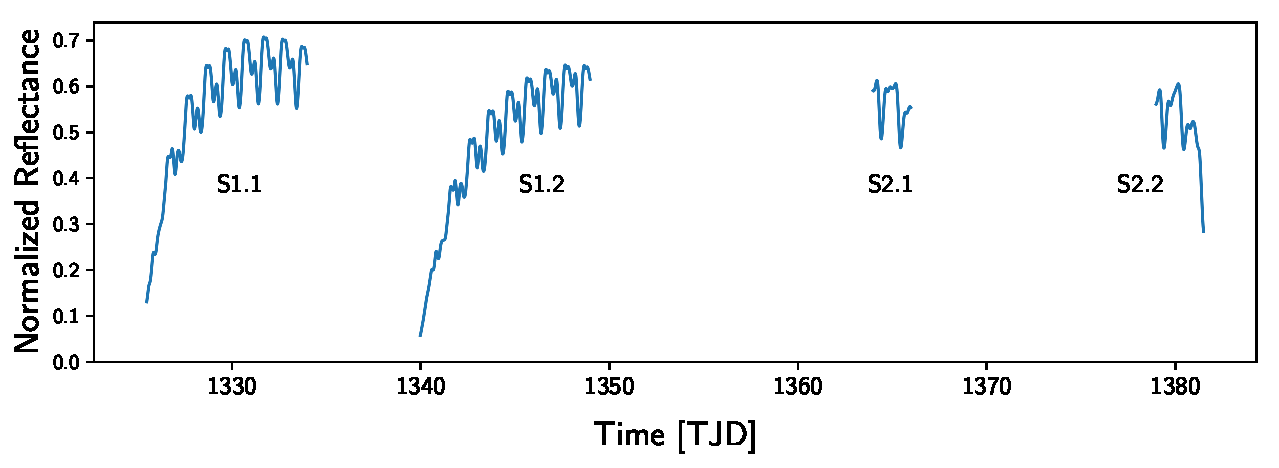
\includegraphics[width=\linewidth]{figures/starry_model.pdf}
    \caption{\label{fig:starry_model}
             Normalized surface reflectance versus time for the maximum
             likelihood \starry model in each of the four orbits of \tess
             in Sectors 1 and 2.
             \codelink{earthshine_S1_S2}
             }
    \end{centering}
\end{figure}

As with the systematics model (\S\ref{sec:systematics}), the model
for the astrophysical signal is \emph{linear}: the signal $\mathbf{s}$ 
is a linear operation on the vector of spherical harmonic coefficients 
$\mathbf{y}$
that describes the body's surface:
%
\begin{align}
    \mathbf{s} = \mathbf{A} \mathbf{y}
\end{align}
%
where $\mathbf{A}$ is the design matrix and $\mathbf{y}$ is the vector of spherical harmonic coefficients. 
Note that in \cite{Luger2019}, $\mathbf{y}$ describes the emissivity of the surface,
but here we will use it to represent the \emph{albedo} of the planet.
We choose a maximum spherical harmonic degree $l_{max} = 10$ for our fits,
noting that increasing $l_{max}$ above this value 
leads to a quick rise in the amount of ``ringing'' without substantially
increasing the quality of our fits. Note that $l = 10$ corresponds to
a maximum surface resolution on the order of $180^\circ/10 \approx 18^\circ$.

Finally, for reference, in Figure~\ref{fig:starry_model} we plot the
\starry model for our maximum likelihood fit (\S\ref{sec:results}). The
sharp rise at the beginning of each orbit in Sector 1 is due to the changing
vantage point of \tess as Sol d transitions from a thin crescent to full phase.

\subsection{Full Model and Likelihood Function}
\label{sec:model}

Our full model for each light curve is simply the product of the 
systematics model $\mathbf{p}_n = \mathbf{B}\mathbf{w}_n$ (different for each target) and
the \starry model $\mathbf{s} = \mathbf{A}\mathbf{y}$ (shared by all targets). Since we happen
to know the exact distance $\mathbf{r}$ between \tess and Sol d at all times
(\S\ref{sec:orbit}), we also include the inverse square of $\mathbf{r}$ 
as a multiplicative term. The model for the flux timeseries
in the $n^\mathrm{th}$ postage stamp is therefore
%
\begin{align}
    \label{eq:model}
    \mathbf{m}_n = (\mathbf{r}^{-2}) \circ (\mathbf{B} \mathbf{w}_n) \circ (\mathbf{A} \mathbf{y})
\end{align}
%
where $\circ$ denotes the element-wise product of two vectors.

We solve Equation~(\ref{eq:model}) for the weights $\mathbf{w}_n$ and $\mathbf{y}$
by maximizing the negative log likelihood function in two separate steps. In the
first step, we take advantage of the linearity of the problem to perform a fast,
semi-analytical optimization to obtain a starting guess for the weights. In the
second step, we apply additional constraints to prevent overfitting and ensure
an albedo in the range $[0, 1]$ everywhere on the surface.

In the first step, we initialize the \starry model to unity and iteratively
solve for $\mathbf{w}_n$ and $\mathbf{y}$ by solving the L2-regularized
least squares problem \citep[see, e.g., \S2.1 in][]{Luger2018a}.
We assume zero-mean Gaussian priors for the weights:
%
\begin{equation}
    \label{eq:wprior}
    \begin{aligned}
        \mathbf{w}_n \sim \mathcal{N}(0, \sigma_w^2)
    \end{aligned}
    \qquad\qquad\qquad\qquad
    \begin{aligned}
        \mathbf{y} \sim \mathcal{N}(0, \sigma_y(l)^2)
    \end{aligned}\, ,
\end{equation}
%
with $\sigma_w = 0.1$ and 
%
\begin{align}
    \sigma_y(l) &=
    \begin{dcases}
        1.75\times 10^{-5} \, l^\frac{3}{2} & 
            \quad\quad\quad\quad\quad\quad\quad\quad\quad\quad 
            l < 2
        \\
        1.40\times 10^{-4} \, l^{-\frac{3}{2}} & 
            \quad\quad\quad\quad\quad\quad\quad\quad\quad\quad 
            l \geq 2
    \end{dcases}
    \, ,
\end{align}
%
where $l$ is the spherical harmonic degree. The latter prior was chosen
by trial-and-error and was adjusted to keep the albedo positive
everywhere on the surface. Note, importantly, that we do
not fit for the coefficient of the constant $Y_{0,0}$ spherical harmonic,
but instead fix it to unity. Since the solutions obtained in this step are merely
used as a starting point for the second step (see below), the choice of prior 
at this stage has minimal impact on our results.

In general, we find that the iterative scheme converges within about 50 
iterations, taking about fifteen minutes on a laptop computer. However, since it 
is strongly regularized, the model significantly
underfits the data. In the second step, we remove our L2 prior on the spherical
harmonic coefficients and instead regularize the actual surface albedo, which
we compute on a uniform spherical grid with 50,000 points. We enforce a 
uniform prior in the range $[0, 1]$, with a small amount of Gaussian smoothing on either 
side. We additionally impose a constraint on the power spectrum of the
inferred map, requiring that it be drawn from a distribution whose mean
is a decaying power law in the spherical harmonic degree $l$ in order
to suppress ringing and spurious high order features.
Our full negative log likelihood function in this step is therefore
%
\begin{align}
    \label{eq:nll}
    -\log\mathcal{L} \, = \, 
        &\frac{1}{2}(\mathbf{f} - \mathbf{m})^\top \boldsymbol{\Sigma}^{-1} (\mathbf{f} - \mathbf{m}) \, + \nonumber \\
        &\frac{1}{2}\mathbf{w}^\top \boldsymbol{\Lambda}_w^{-1} \mathbf{w} \, + \nonumber \\
        &\frac{1}{2}(\mathbf{a_-} + 1 - \mathbf{a_+})^\top \boldsymbol{\Lambda}_a^{-1} (\mathbf{a_-} + 1 - \mathbf{a_+}) \, + \nonumber \\
        &\frac{1}{2}(\boldsymbol{\rho} - \boldsymbol{l}^{-\gamma})^\top \boldsymbol{\Lambda}_\rho^{-1} (\boldsymbol{\rho} - \boldsymbol{l}^{-\gamma}) \, + \nonumber \\
        &\frac{1}{2} \frac{(\gamma - \gamma_0)^2}{\sigma_\gamma^2}
        \quad,
\end{align}
%
where $\mathbf{f}$ is the measured flux across all targets,
$\mathbf{m}$ is the full model (Equation~\ref{eq:model}),
$\boldsymbol{\Sigma}$ is the (diagonal) data covariance, 
$\mathbf{w}$ are the systematics model weights for all targets,
$\boldsymbol{\Lambda}_w$ is the prior covariance of the weights
(Equation~\ref{eq:wprior}), $\mathbf{a_-}$ and $\mathbf{a_+}$ are
vectors containing the values of the albedo that are below zero and above one, 
respectively, $\boldsymbol{\Lambda}_a$ is the covariance of the Gaussian
used to smooth the edges of the top-hat prior on $\mathbf{a}$,
$\boldsymbol{\rho}$ is the power spectrum of the inferred spherical harmonic map
(equal to the sum of the squares of the coefficients at each degree $\boldsymbol{l}$),
$\gamma$ is the power law index of the power spectrum prior, $\boldsymbol{\Lambda}_\rho$ is the
covariance of that prior, $\gamma_0 = 1.5$ is the mean of the prior on $\gamma$
and $\sigma_\gamma^2 = 10^{-2}$ is the corresponding variance.
%
For simplicity, all our prior covariances are diagonal and
homoscedastic with variances equal to $2.5\times 10^{-3}$ for $\mathbf{w}$, and
$10^{-8}$ for $\mathbf{a}$, $10^{-1}$ for $\boldsymbol{\rho}$.

Unfortunately, the constraints outlined above break the linearity 
of the problem, and we must turn to a non-linear optimizer. We use the 
\textsf{AdamOptimizer} method in the \tf package \citep{Abadi2015}
to maximize Equation~(\ref{eq:nll}). Starting with the values of the
weights obtained in the first step, we run the \textsf{AdamOptimizer}
for 1000 iterations, well past convergence. Since \tf automatically
computes and propagates gradient information, this step is fast
and also finishes in under five minutes on a standard computer.

\section{Results}
\label{sec:results}

\begin{figure}[t!]
    \begin{centering}
    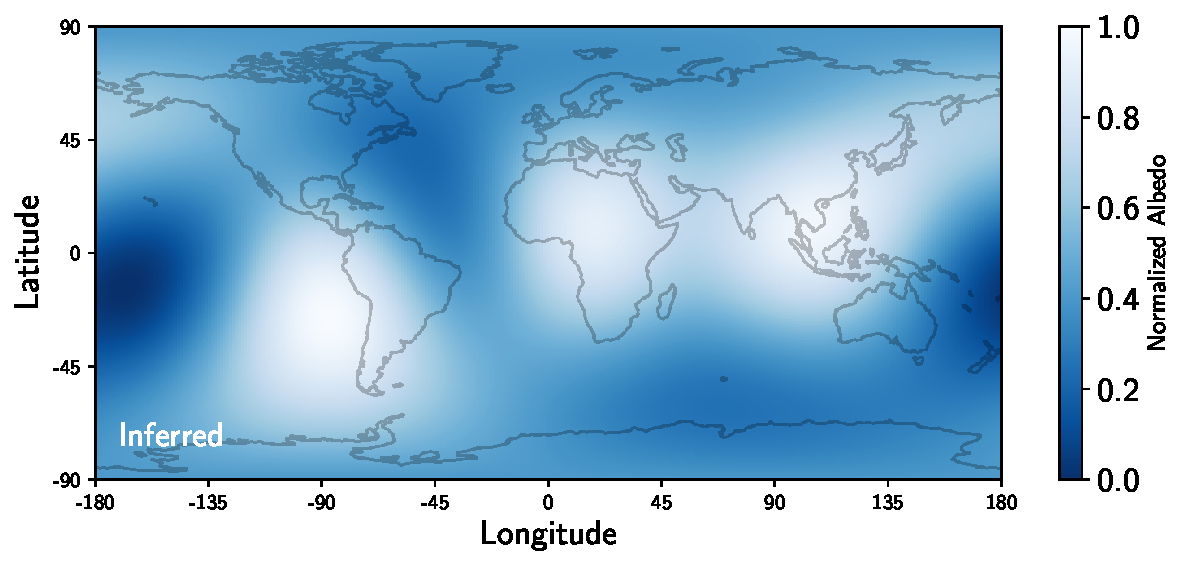
\includegraphics[width=\linewidth]{figures/map_L2.pdf}
    \caption{\label{fig:map_L2}
             Maximum likelihood map of Sol d obtained during the first
             stage of our optimization procedure, in which an iterative
             analytic approach was used to solve the bilinear model, 
             subject to very conservative regularization. Despite the low
             resolution of this map, the bright features appear to track
             land masses which for specificity we will refer to as (from left to right)
             ``South America,'' ``Africa,'' and ``Asia.''
             The two dark features are associated with the planet's
             two purported oceans, which we call the ``Pacific'' and the ``Atlantic.''
             }
    \end{centering}
\end{figure}

Figure~\ref{fig:map_L2} shows the maximum likelihood map inferred
during the first stage of our optimization procedure. Since the map
coefficients were heavily regularized, the dynamic range of the albedo
variations was less than 10\%; we scaled it to span the range [0, 1]
for better visualization. Furthermore, although the resolution is on 
the order of $12^\circ$, features typically span ${\sim}45^\circ$; this is
also an artefact of our regularization. However, broad features are already
visible in the map: three bright regions and two dark regions (one of which
wraps around the antimeridian). Overplotted on the inferred map are
coastal outlines corresponding to our current best understanding of 
the geography of Sol d. One can see that the three bright regions roughly
track, from left to right, continents we shall refer to as ``South America,''
``Africa,'' and ``Asia,'' in keeping with the literature. The dark regions
are associated with the two major purported oceans on the planet, the
``Pacific'' (centered at longitude $\pm180^\circ$) and ``Atlantic''
(centered at longitude $\-45^\circ$).

\begin{figure}[t!]
    \begin{centering}
    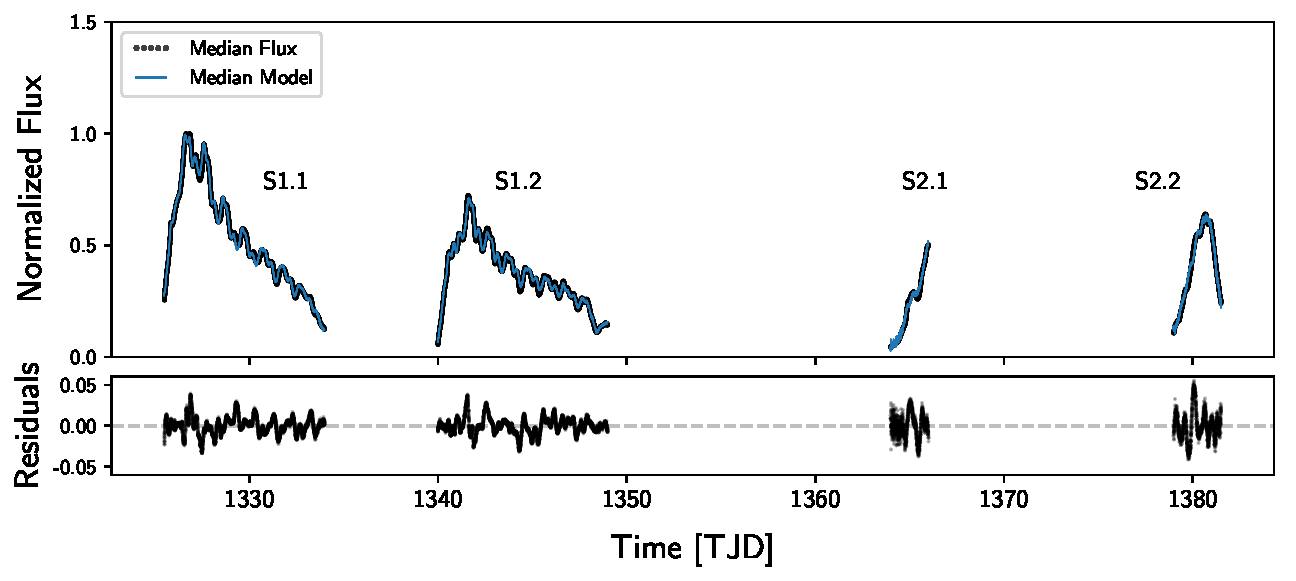
\includegraphics[width=\linewidth]{figures/model.pdf}
    \caption{\label{fig:model}
             \emph{Top:} Median flux across all postage stamps (black) and
             the median maximum likelihood model (blue) across Sectors 1 and 2.
             \emph{Bottom:} Median residuals about the maximum likelihood fit.
             \codelink{earthshine_S1_S2}
             }
    \end{centering}
\end{figure}

As expected, the second, non-linear step in our optimization procedure
yields a much better fit to the data.
The top panel of Figure~\ref{fig:model} shows the median of the 
maximum likelihood model in this second step
across all 95 targets (blue) overplotted on the median flux (black). 
The median residuals are shown in the bottom panel; these have
standard deviation of less than one percent. While there is significant correlated
structure in the residuals, their power spectrum displays a broad peak extending 
between about 0.1 and 10 days, with a significant dip at 1.00 day. This
suggests our model is fitting the rotational variability of Sol d quite well, but
additional temporal variations---most likely due to cloud movement---cause aperiodic
changes to the reflectivity of the surface. We revisit this point in \S\ref{sec:discussion}.

\begin{figure}[p!]
    \begin{centering}
    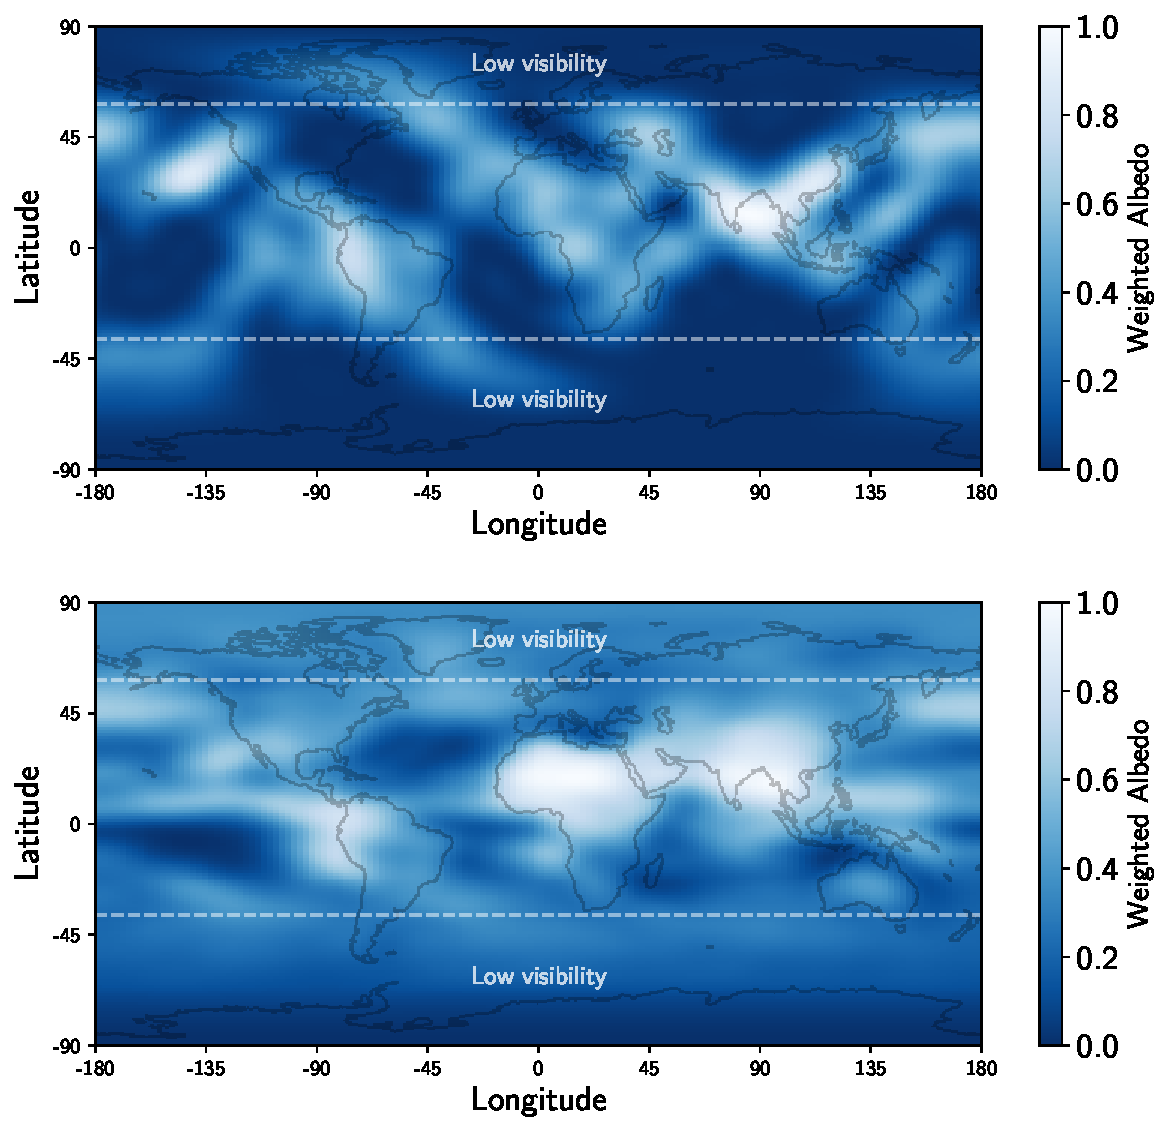
\includegraphics[width=\linewidth]{figures/map.pdf}
    \caption{\label{fig:map}
             \emph{Top:} The maximum likelihood model for the surface albedo
             of Sol d, weighted by the visibility across Sectors 1 and 2. The
             dashed white lines indicate latitudes above/below which the
             visibility drops below 50\%. Black contours indicate coastlines
             derived from current state-of-the-art models of the surface geography 
             of Sol d.
             \emph{Bottom:} Approximate cloud coverage map based on corrected
             surface reflectance obtained by the
             \emph{VIIRS} imager, averaged over the same date range and weighted
             by the same visibility function.
             \codelink{earthshine_S1_S2}
             }
    \end{centering}
\end{figure}

In the top panel of Figure~\ref{fig:map} we show the final,
maximum likelihood albedo map inferred for Sol d weighted by a visibility function.
The visibiluty function is computed as the average of the product of the 
cosine of the illumination angle and the cosine of the angle between the 
observer vector and the vector normal to the surface of Sol d. This normalization
has the effect of downweighting regions that are either seldom illuminated (such
as regions near the southern pole of Sol d, as the observations were taken during
southern winter) or seldom in view (such as regions near the north pole of the planet,
which during Sectors 1 and 2 were mostly on the opposite side of Sol d than \tess).
Because there is little data from these regions, their albedo is prior-dominated
and tends to fluctuate substantially with small changes to the choices we make
when fitting the data. Conversely, we find that the large scale features close to
the equator of Sol d are mostly insensitive to our choices of prior. In the Figure,
we use dashed lines to delineate the regions whose average visibility is larger
than 0.5.

The bottom panel of Figure~\ref{fig:map} shows an approximate average
cloud cover map of Sol d based on imagery taken by the
Visible Infrared Imaging Radiometer Suite (\emph{VIIRS}) instrument aboard the 
Suomi National Polar-orbiting Partnership (\emph{S-NPP}) satellite%
\footnote{Data obtained via 
\href{https://github.com/rodluger/earthshine/blob/master/tex/figures/viirs.sh}{this wget script}.}. 
The image was produced by analyzing the corrected true color reflectance in the
I1 (red), M4 (blue), and M3 (green) bands and masking
all pixels that were either dark or had significant variance among the three
bands (i.e., inconsistent with a grey spectrum). We then averaged the images
averaged over the 28 days of data analyzed in this work, smoothed it, 
and weighted by the \tess visibility as in the top panel.

While the two panels display fundamentally different quantities---an albedo
and a cloudiness factor---we expect that the signal of Sol d in the \tess
bandpass is dominated by cloud reflectivity, as water clouds have an albedo
higher than soil, vegetation, or ocean in the optical/near infrared
\citep[e.g.,][]{Jedlovec2009}. We therefore
expect large, coherent cloud structures to show up as the brightest regions 
in our inferred map, and in fact we find that this is generally the case. The
dominant feature in our inferred map is a bright region spanning longitudes
of $+50^\circ$ to $+100^\circ$ just northward of the equator. This is also the
dominant feature in the VIIRS map, corresponding to the persistent weather system
associated with summertime monsoons in the south of Asia.

Secondary features common to both maps are a permanent cloudy region over
central Africa with a westward spur over the Atlantic Ocean, a veneer of clouds
over the north Pacific, and a pile up of clouds on the western coast of
northern South America. The dark regions in the inferred map rather loosely
track the Pacific, Atlantic, and Indian Oceans, although the correspondence
is not exact.

\section{Discussion}
\label{sec:discussion}

The problem of inferring a two-dimensional map from a one-dimensional
timeseries is famously ill-posed given its large null space and many complex
degeneracies \citep[e.g.,][]{CowanFuentesHaggard2013}. In fact, for a 
uniformly illuminated body, its rotational light curve encodes at most
$2l_\mathrm{max}$ modes (one sine term and one cosine term per frequency), 
where $l_\mathrm{max}$ is the highest spherical
harmonic degree of features on the surface of the body. The number of modes
\emph{on the surface of the body}, however, increases quadratically 
as $(l_\mathrm{max} + 1)^2$. This means that for a body whose surface is
perfectly described by a spherical harmonic map of degree $l_\mathrm{max} = 10$,
which is described by 121 coefficients, only 20 linear combinations
of those coefficients are actually projected onto the light curve. The
problem is fundamentally non-invertible, since most of the information
one wishes to extract lies in the null space.

Fortunately, there are two aspects of the problem at hand that facilitate
this (seemingly impossible) inversion. First, the surface of Sol d is
not uniformly illuminated; instead, different parts of the surface are weighted
by different amounts as the planet rotates and as the angle of incident starlight
moves over the course of the year. This weighting is sufficient to break many
of the degeneracies, which are rooted in the anti-symmetry of many of the spherical
harmonic modes. Moreover, the discontinuous day/night terminator further
breaks these degeneracies, as only modes that are anti-symmetric about
the visible lune of the planet strictly remain in the null space. Second, 
the changing vantage point of \tess relative to Sol d (and our exact knowledge of it)
break degeneracies that are viewpoint-dependent. In particular, the motion of
\tess changes the position and shape of the terminator on the projected disk
of Sol d, enhancing the effect discussed above.

In fact, because of these points, there should formally be \emph{no} null space 
in this particular problem. In practice, however, it is evident from
Figure~\ref{fig:map} that degenaricies still abound. \todo{bla bla bla.}

\subsection{Temporal Evolution}

Residuals in Figure~\ref{fig:model} display significant correlated
structure. Talk about their power spectrum. Talk about how S2 is worse fit.

\begin{figure}[p!]
    \begin{centering}
    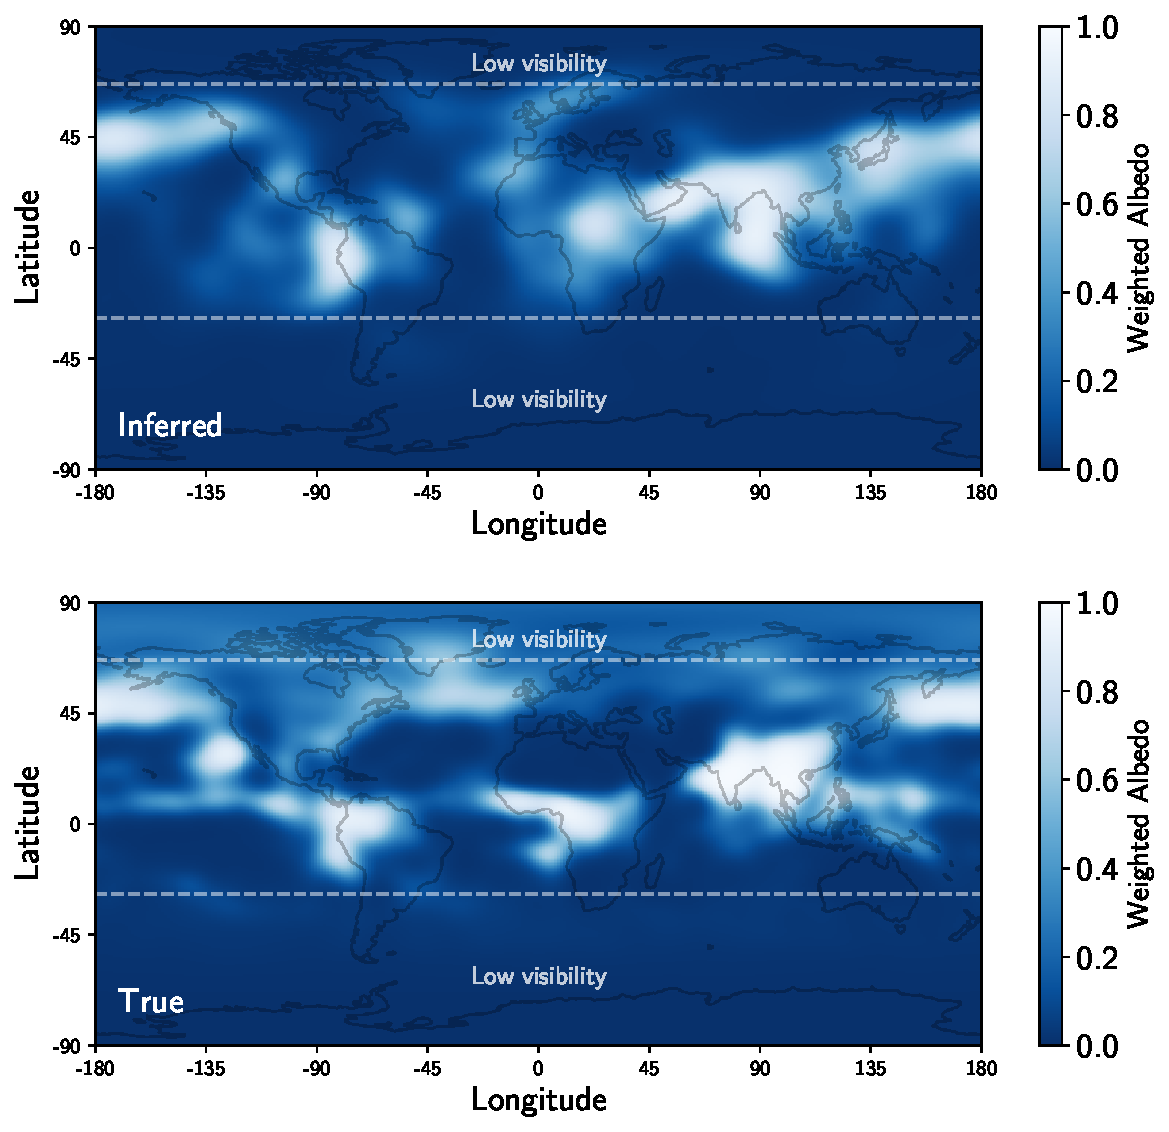
\includegraphics[width=\linewidth]{figures/map_temporal.pdf}
    \caption{\label{fig:map_temporal}
             The inferred mean map when allowing for slight temporal
             variations in the spherical harmonic coefficients. Compare
             to Figure~\ref{fig:map}. An animated version of this figure
             is available on 
             \href{https://github.com/rodluger/earthshine/blob/master/tex/figures/map_temporal.mp4}{GitHub}.
             \codelink{earthshine_S1_S2}
             }
    \end{centering}
\end{figure}

\subsection{Sources of Bias}

In our analysis, we neglected the effects of limb darkening. Because of
atmospheric attenuation, features near the limb of the planet should in
reality contribute less to the flux than our model predicts. This could
bias our results particularly in cases where the planet is seen at half
phase (for instance, during days 1326 and 1341 in Figure~\ref{fig:phases}).
In the absence of limb darkening, the brightest regions on the planet are those
close to the sub-stellar point, which is on the limb. Limb darkening should
shift the regions of peak brightness closer to the center of the planet, adding
an east-west bias in the location of the features we identify.

We also ignored the finite angular size of Sol at Sol d (about $0.5^\circ$),
treating it instead as a point source. Regions immediately nightward of the 
terminator should therefore contribute a small amount of flux, which we neglect.
The effect, however, is below the resolution of our inferred map, so we expect
it does not introduce significant bias.

Finally, we implicitly assumed an isotropic prior on the spherical harmonic
coefficients by imposing a power spectrum in only the degree $l$. This has the
effect of lessening the extent to which features can be confined to certain
latitudes. In particular, our prior implicitly disfavors banded cloud structure,
which one may \emph{a priori} expect on a rapidly rotating planet such as 
Sol d. The bottom panel of Figure~\ref{fig:map} shows such banded structure
at the equator and at mid-latitudes due to the combined effects of 
north-south circulation and deflection by the Coriolis force.




% \begin{figure}[t!]
%     \begin{centering}
%     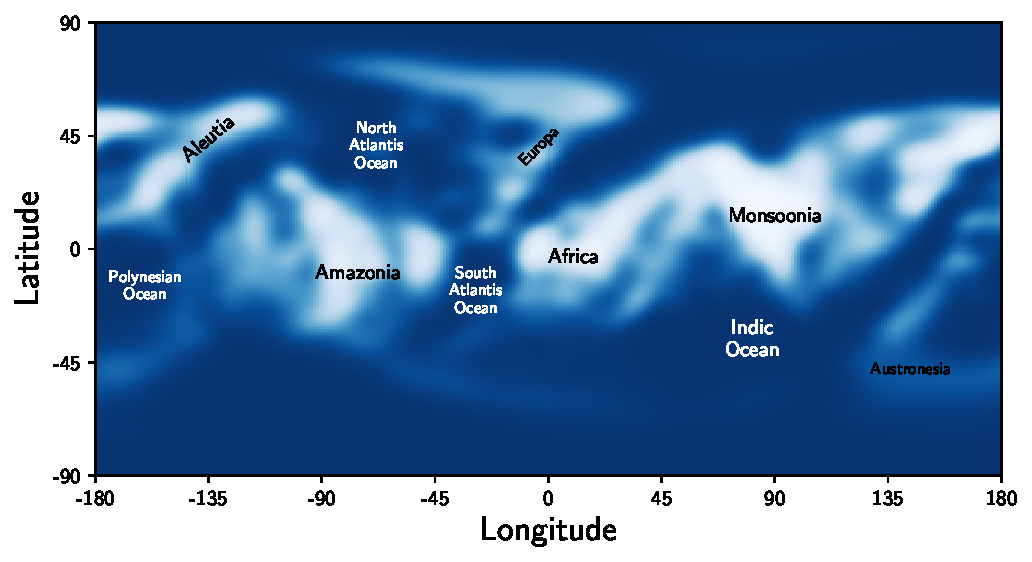
\includegraphics[width=\linewidth]{figures/map_labels.pdf}
%     \caption{\label{fig:map_labels}
%             Map of Sol d with the major features indicated with suggested
%             names.
%             \codelink{earthshine_S1_S2}
%             }
%     \end{centering}
% \end{figure}

\todo{(comparison of inferred features to ``model'' (Earth))}

\todo{No zonal cloud bands: prior.}

\section{Conclusion}
\label{sec:conclusion}

\todo{(summarize)}

\todo{(utility for \TESS background removal)}

\todo{(talk abt prospects for doing this analysis with exoplanets)}


\acknowledgements{\todo{(Artist acknowledgement)} The authors gratefully 
acknowledge Dan Foreman-Mackey, David W Hogg, Ben Pope, \todo{and ...} 
for useful conversations. Crucial parts of this work were carried out at the 
TESS Data Workshop, hosted by Space Telescope Science Institute, and the 
Building Early Science with TESS Workshop, hosted by the University of Chicago.}
\facility{TESS}
\software{Astropy, Matplotlib, Numpy, \starry \citep{Luger2019}, 
TensorFlow \citep{Abadi2015}, \spiceypy \citep{Annex2019}}
% Bibliography
\pagebreak
\bibliography{bib}

\end{document}
